% Options for packages loaded elsewhere
\PassOptionsToPackage{unicode}{hyperref}
\PassOptionsToPackage{hyphens}{url}
%
\documentclass[
  english,
  man,floatsintext]{apa7}
\usepackage{lmodern}
\usepackage{amssymb,amsmath}
\usepackage{ifxetex,ifluatex}
\ifnum 0\ifxetex 1\fi\ifluatex 1\fi=0 % if pdftex
  \usepackage[T1]{fontenc}
  \usepackage[utf8]{inputenc}
  \usepackage{textcomp} % provide euro and other symbols
\else % if luatex or xetex
  \usepackage{unicode-math}
  \defaultfontfeatures{Scale=MatchLowercase}
  \defaultfontfeatures[\rmfamily]{Ligatures=TeX,Scale=1}
\fi
% Use upquote if available, for straight quotes in verbatim environments
\IfFileExists{upquote.sty}{\usepackage{upquote}}{}
\IfFileExists{microtype.sty}{% use microtype if available
  \usepackage[]{microtype}
  \UseMicrotypeSet[protrusion]{basicmath} % disable protrusion for tt fonts
}{}
\makeatletter
\@ifundefined{KOMAClassName}{% if non-KOMA class
  \IfFileExists{parskip.sty}{%
    \usepackage{parskip}
  }{% else
    \setlength{\parindent}{0pt}
    \setlength{\parskip}{6pt plus 2pt minus 1pt}}
}{% if KOMA class
  \KOMAoptions{parskip=half}}
\makeatother
\usepackage{xcolor}
\IfFileExists{xurl.sty}{\usepackage{xurl}}{} % add URL line breaks if available
\IfFileExists{bookmark.sty}{\usepackage{bookmark}}{\usepackage{hyperref}}
\hypersetup{
  pdftitle={Dependency learning: comparing adults and children},
  pdflang={en-EN},
  hidelinks,
  pdfcreator={LaTeX via pandoc}}
\urlstyle{same} % disable monospaced font for URLs
\usepackage{graphicx}
\makeatletter
\def\maxwidth{\ifdim\Gin@nat@width>\linewidth\linewidth\else\Gin@nat@width\fi}
\def\maxheight{\ifdim\Gin@nat@height>\textheight\textheight\else\Gin@nat@height\fi}
\makeatother
% Scale images if necessary, so that they will not overflow the page
% margins by default, and it is still possible to overwrite the defaults
% using explicit options in \includegraphics[width, height, ...]{}
\setkeys{Gin}{width=\maxwidth,height=\maxheight,keepaspectratio}
% Set default figure placement to htbp
\makeatletter
\def\fps@figure{htbp}
\makeatother
\setlength{\emergencystretch}{3em} % prevent overfull lines
\providecommand{\tightlist}{%
  \setlength{\itemsep}{0pt}\setlength{\parskip}{0pt}}
\setcounter{secnumdepth}{-\maxdimen} % remove section numbering
% Make \paragraph and \subparagraph free-standing
\ifx\paragraph\undefined\else
  \let\oldparagraph\paragraph
  \renewcommand{\paragraph}[1]{\oldparagraph{#1}\mbox{}}
\fi
\ifx\subparagraph\undefined\else
  \let\oldsubparagraph\subparagraph
  \renewcommand{\subparagraph}[1]{\oldsubparagraph{#1}\mbox{}}
\fi
% Manuscript styling
\usepackage{upgreek}
\captionsetup{font=singlespacing,justification=justified}

% Table formatting
\usepackage{longtable}
\usepackage{lscape}
% \usepackage[counterclockwise]{rotating}   % Landscape page setup for large tables
\usepackage{multirow}		% Table styling
\usepackage{tabularx}		% Control Column width
\usepackage[flushleft]{threeparttable}	% Allows for three part tables with a specified notes section
\usepackage{threeparttablex}            % Lets threeparttable work with longtable

% Create new environments so endfloat can handle them
% \newenvironment{ltable}
%   {\begin{landscape}\begin{center}\begin{threeparttable}}
%   {\end{threeparttable}\end{center}\end{landscape}}
\newenvironment{lltable}{\begin{landscape}\begin{center}\begin{ThreePartTable}}{\end{ThreePartTable}\end{center}\end{landscape}}

% Enables adjusting longtable caption width to table width
% Solution found at http://golatex.de/longtable-mit-caption-so-breit-wie-die-tabelle-t15767.html
\makeatletter
\newcommand\LastLTentrywidth{1em}
\newlength\longtablewidth
\setlength{\longtablewidth}{1in}
\newcommand{\getlongtablewidth}{\begingroup \ifcsname LT@\roman{LT@tables}\endcsname \global\longtablewidth=0pt \renewcommand{\LT@entry}[2]{\global\advance\longtablewidth by ##2\relax\gdef\LastLTentrywidth{##2}}\@nameuse{LT@\roman{LT@tables}} \fi \endgroup}

% \setlength{\parindent}{0.5in}
% \setlength{\parskip}{0pt plus 0pt minus 0pt}

% \usepackage{etoolbox}
\makeatletter
\patchcmd{\HyOrg@maketitle}
  {\section{\normalfont\normalsize\abstractname}}
  {\section*{\normalfont\normalsize\abstractname}}
  {}{\typeout{Failed to patch abstract.}}
\makeatother
\shorttitle{Dependency learning}
\author{Jens Roeser\textsuperscript{1}}
\affiliation{
\vspace{0.5cm}
\textsuperscript{1} Department of Psychology, Nottingham Trent University, United Kingdom}
\authornote{

Correspondence concerning this article should be addressed to Jens Roeser, 50 Shakespeare St, Nottingham NG1 4FQ. E-mail: jens.roeser@ntu.ac.uk}
\keywords{}
\usepackage{csquotes}
\usepackage{booktabs}
\usepackage{longtable}
\usepackage{graphicx}
\usepackage{array}
\usepackage{float}
\usepackage{threeparttable}
\usepackage[normalem]{ulem}
\usepackage[utf8]{inputenc}
\usepackage{icomma}
\ifxetex
  % Load polyglossia as late as possible: uses bidi with RTL langages (e.g. Hebrew, Arabic)
  \usepackage{polyglossia}
  \setmainlanguage[]{english}
\else
  \usepackage[shorthands=off,main=english]{babel}
\fi
\ifluatex
  \usepackage{selnolig}  % disable illegal ligatures
\fi
\newlength{\cslhangindent}
\setlength{\cslhangindent}{1.5em}
\newenvironment{cslreferences}%
  {\setlength{\parindent}{0pt}%
  \everypar{\setlength{\hangindent}{\cslhangindent}}\ignorespaces}%
  {\par}

\title{Dependency learning: comparing adults and children}

\date{}

\begin{document}
\maketitle

\hypertarget{comparisons-between-children-and-adults}{%
\section{Comparisons between children and adults}\label{comparisons-between-children-and-adults}}

In this final analysis we evaluate differences between the adults (Experiment 1) and the children results (Experiment 2). In particular, we focused on the effect of main interest to evaluate implicit learning; i.e.~the slowdown in reaction times in the transfer block (Block 7) relative to Block 6. Also we tested for learning differences comparing the conditional effects for Block 1 and Block 6; we observed evidence for learning differences in the results section of Experiment 1 and Experiment 2. To compared the data from adults and children we pooled the serial reaction-time data from both experiments and extracted the data from Blocks 1, 6 and 7.

This analysis was largely similar to the reaction-time models reported earlier: reaction times were modelled in Bayesian linear mixed-effects models. Reaction times for elements that were not part of an adjacent or nonadjacent dependency were included in the model as baseline. Model predictors were Age Group (levels: adults, children), Dependency (levels: dependency, baseline), Adjacency (levels: adjacent, nonadjacent), Learning Block (levels: 1, 6), Transfer Block (levels: 6, 7), and all by-Dependency and by-Adjacency interactions with Group and Block. All predictors were sum-coded following Schad et al. (2020). Reaction time data were fitted with a shifted-lognormal distribution, random intercepts for each stimulus image, and participants with by-participant slope adjustments for all main effects and interactions.

In addition to the parameter estimates as in the previous results sections, we used the posterior to calculate the standardised effect sizes \(\delta\), defined as \(\delta = \frac{\mu}{\sigma}\) , where \(\mu\) is the parameter value of the effect of interest and \(\sigma\) is the standard deviation. The effect size was calculated to allow comparisons across age group (Wagenmakers et al., 2010). Because the standard deviation is necessary to calculate the effect size, we specified the model with two different variance components, one for the children group and one for the adults group as the population standard deviation is likely to be different for each group (Baguley, 2009).

For the effect sizes, we determined the region of practical equivalence (henceforth, ROPE) to assess the uncertainty of the effect size (Makowski et al., 2019). The ROPE is the range of values that are practically equivalent to a null effect (see e.g.~Kruschke, 2010, 2011). For the effect size we set the ROPE to be -0.1 and 0.1 (Kruschke, 2018) which is the range of negligible effect sizes (Cohn, 1988). The value returned is the proportion of posterior samples (of the effect size) that falls inside the ROPE. In other words, the ROPE value indicates the extent to which the posterior cannot rule out an negligible effect. A meaningful effect size should have a small proportion of posterior samples within the ROPE.

Table \ref{tab:tablemodel} summaries the modelling outcome for the serial reaction-time data. We found compelling evidence for longer reaction times for children compared to adults. Also, overall we found evidence that adjacent dependencies were responded to faster than nonadjacent dependencies. Reaction times for Block 6 were shorter than for Block 1 and were followed by a slowdown for Block 7. Further evidence was found for two-way interactions of Age Group and Dependency, and Age Group and Learning Block. Importantly, we found evidence for a three-way interaction of Dependency by Transfer Block and Age Group. The variance of the children group \(\sigma_{children}\) was larger than the variance of the adults group \(\sigma_{adults}\). There was negligible evidence for all remaining predictors.

\begin{center}
\begin{ThreePartTable}

\begin{TableNotes}[para]
\normalsize{\textit{Note.} $\hat{\mu}$ = most probable parameter value; 95\% HPDI = interval containing 95\% of the probability mass; $P(\hat{\mu}<0)$ = probability of the true parameter value being smaller than 0; $\times$ = interaction.}
\end{TableNotes}

\small{

\begin{longtable}{lrrr}\noalign{\getlongtablewidth\global\LTcapwidth=\longtablewidth}
\caption{\label{tab:tablemodel}Age-group comparison for serial reaction-time data. Estimated parameter values (in msecs) for main effects and interactions of Learning Block (levels: 1, 6) and Transfer Block (levels: 6, 7), Age Group (levels: adults, children), Dependency (levels: dependency, baseline), Adjacency (levels: adjacent, nonadjacent).}\\
\toprule
Predictor & \multicolumn{1}{c}{$\hat{\mu}$} & \multicolumn{1}{c}{95\% HPDI} & \multicolumn{1}{c}{$P(\hat{\mu}<0)$}\\
\midrule
\endfirsthead
\caption*{\normalfont{Table \ref{tab:tablemodel} continued}}\\
\toprule
Predictor & \multicolumn{1}{c}{$\hat{\mu}$} & \multicolumn{1}{c}{95\% HPDI} & \multicolumn{1}{c}{$P(\hat{\mu}<0)$}\\
\midrule
\endhead
Main effects &  &  & \\
\ \ \ Age Group & -327 & [-383, -270] & >.999\\
\ \ \ Dependency & 3 & [-30, 34] & .447\\
\ \ \ Adjacency & -23 & [-41, 0] & .977\\
\ \ \ Block: Learning & 217 & [189, 243] & <.001\\
\ \ \ Block: Transfer & -35 & [-54, -19] & >.999\\
Two-way interactions &  &  & \\
\ \ \ Age $\times$ Dependency & -64 & [-88, -41] & >.999\\
\ \ \ Age $\times$ Adjacency & -12 & [-30, 8] & .877\\
\ \ \ Age $\times$ Block (Learning) & 69 & [49, 92] & <.001\\
\ \ \ Age $\times$ Block (Transfer) & -2 & [-18, 13] & .616\\
\ \ \ Dependency $\times$ Block (Learning) & 4 & [-11, 22] & .278\\
\ \ \ Dependency $\times$ Block (Transfer) & -16 & [-40, 5] & .928\\
\ \ \ Adjacency $\times$ Block (Learning) & -6 & [-19, 8] & .757\\
\ \ \ Adjacency $\times$ Block (Transfer) & 2 & [-14, 19] & .415\\
Three-way interactions &  &  & \\
\ \ \ Dependency $\times$ Block (Learning) $\times$ Age & -3 & [-19, 14] & .618\\
\ \ \ Dependency $\times$ Block (Transfer) $\times$ Age & -25 & [-41, -7] & .997\\
\ \ \ Adjacency $\times$ Block (Learning) $\times$ Age & 3 & [-11, 17] & .327\\
\ \ \ Adjacency $\times$ Block (Transfer) $\times$ Age & -1 & [-14, 15] & .499\\
Variance components &  &  & \\
\ \ \ $\sigma_{adults}$ & 0.32 & [0.31, 0.32] & --\\
\ \ \ $\sigma_{children}$ & 0.37 & [0.36, 0.38] & --\\
\bottomrule
\addlinespace
\insertTableNotes
\end{longtable}

}

\end{ThreePartTable}
\end{center}

Figure \ref{fig:plotgroupcomp} illustrates the modelled serial reaction-time data illustrating the speedup from Block 1 to Block 6 and the slowdown from Block 6 to Block 7 for the adult and the children group. The slowdown from Block 6 to 7 was tested within Age Group and Dependency to gain further insight into the source of the three-way interaction. Reported are the effect sizes for each comparison.

\begin{figure}[ht]

{\centering 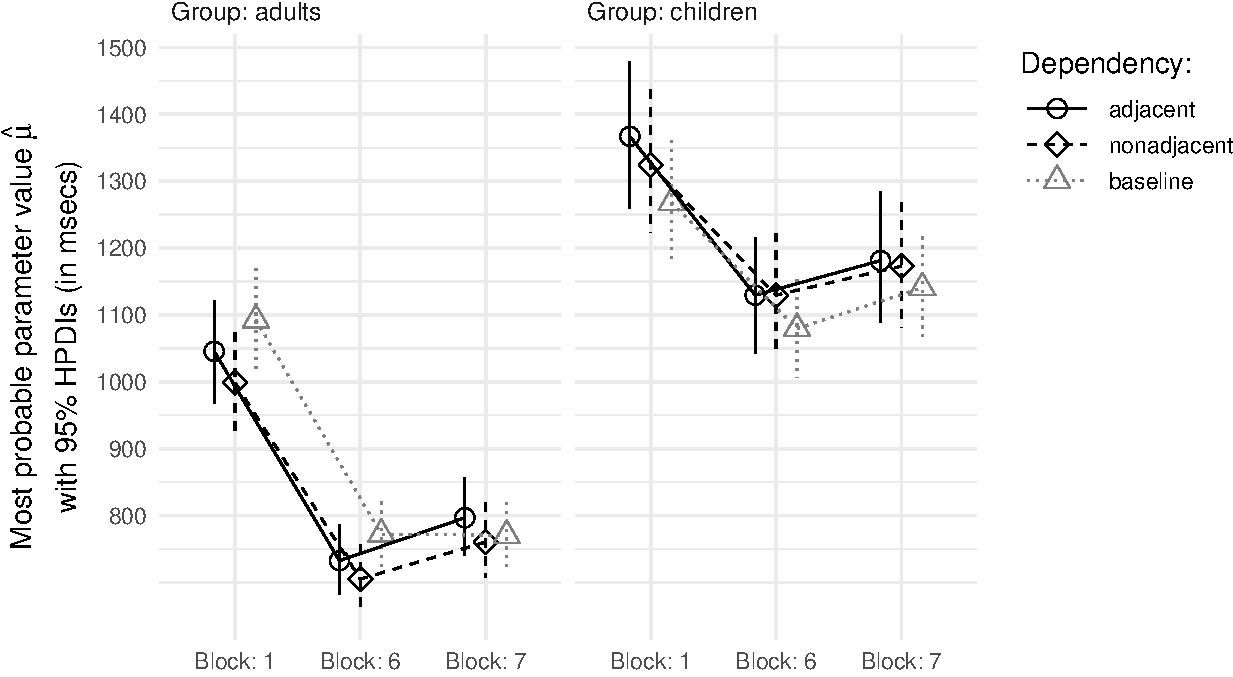
\includegraphics{Group-comparison_v3_files/figure-latex/plotgroupcomp-1} 

}

\caption{Modelled serial reaction-time data (group comparison). Reaction-time data are shown by age group for the first block compared to Block 6 (learning) and Block 6 compared to the final block (transfer). Shown are the modelled reaction-time data with 95\% HPDI (in msecs) for both adjacency conditions (adjacent, nonadjacent) and the baseline condition.}\label{fig:plotgroupcomp}
\end{figure}

We observed an interaction of Dependency (levels: dependency, baseline), Transfer Block (levels: 6 and 7), and Age Group. For the adult group, we observed a small effect for a slowdown from Block 6 to 7 in the dependency condition (\(\hat{\delta}\) = 0.25, 95\% HPDI{[}0.11, 0.39{]}, ROPE = 0) but negligible evidence for a slowdown in baseline trials (\(\hat{\delta}\) = -0.01, 95\% HPDI{[}-0.08, 0.07{]}, ROPE = 100\%). For the children group, we observed a negligible slowdown effect in the dependency condition (\(\hat{\delta}\) = 0.11, 95\% HPDI{[}-0.02, 0.25{]}, ROPE = 42.53) and a small slowdown effect for the baseline condition (\(\hat{\delta}\) = 0.14, 95\% HPDI{[}0.07, 0.23{]}, ROPE = 6\%).

\newpage

\hypertarget{references}{%
\section{References}\label{references}}

\begingroup
\setlength{\parindent}{-0.5in}
\setlength{\leftskip}{0.5in}

\hypertarget{ref}{}

\endgroup

\hypertarget{refs}{}
\begin{cslreferences}
\leavevmode\hypertarget{ref-baguley2009standardized}{}%
Baguley, T. (2009). Standardized or simple effect size: What should be reported? \emph{British Journal of Psychology}, \emph{100}(3), 603--617.

\leavevmode\hypertarget{ref-cohn1988statistical}{}%
Cohn, J. (1988). \emph{Statistical power analysis for the behavioral sciences}. Lawrence Earlbam Associates.

\leavevmode\hypertarget{ref-kruschke2010believe}{}%
Kruschke, J. K. (2010). What to believe: Bayesian methods for data analysis. \emph{Trends in Cognitive Sciences}, \emph{14}(7), 293--300.

\leavevmode\hypertarget{ref-kruschke2011bayesian}{}%
Kruschke, J. K. (2011). Bayesian assessment of null values via parameter estimation and model comparison. \emph{Perspectives on Psychological Science}, \emph{6}(3), 299--312.

\leavevmode\hypertarget{ref-kruschke2018rejecting}{}%
Kruschke, J. K. (2018). Rejecting or accepting parameter values in Bayesian estimation. \emph{Advances in Methods and Practices in Psychological Science}, \emph{1}(2), 270--280.

\leavevmode\hypertarget{ref-makowski2019bayestestr}{}%
Makowski, D., Ben-Shachar, M. S., \& Lüdecke, D. (2019). bayestestR: Describing effects and their uncertainty, existence and significance within the Bayesian framework. \emph{Journal of Open Source Software}, \emph{4}(40), 1541.

\leavevmode\hypertarget{ref-schad2020capitalize}{}%
Schad, D. J., Vasishth, S., Hohenstein, S., \& Kliegl, R. (2020). How to capitalize on a priori contrasts in linear (mixed) models: A tutorial. \emph{Journal of Memory and Language}, \emph{110}, 104038.

\leavevmode\hypertarget{ref-wagenmakers2010bayesian}{}%
Wagenmakers, E.-J., Lodewyckx, T., Kuriyal, H., \& Grasman, R. (2010). Bayesian hypothesis testing for psychologists: A tutorial on the Savage-Dickey method. \emph{Cognitive Psychology}, \emph{60}(3), 158--189.
\end{cslreferences}

\end{document}
